\section{Observation model}
\label{sec:observationModel}
Figure \ref{fig:observModel} gives an overview of the Observation Model as implemented in the current version of PharmML, which covers only continuous data models. A future release will cover discrete data models, such as categorical, count and time-to-event (greyed out in the figure).
\begin{figure}[h!]
\centering
 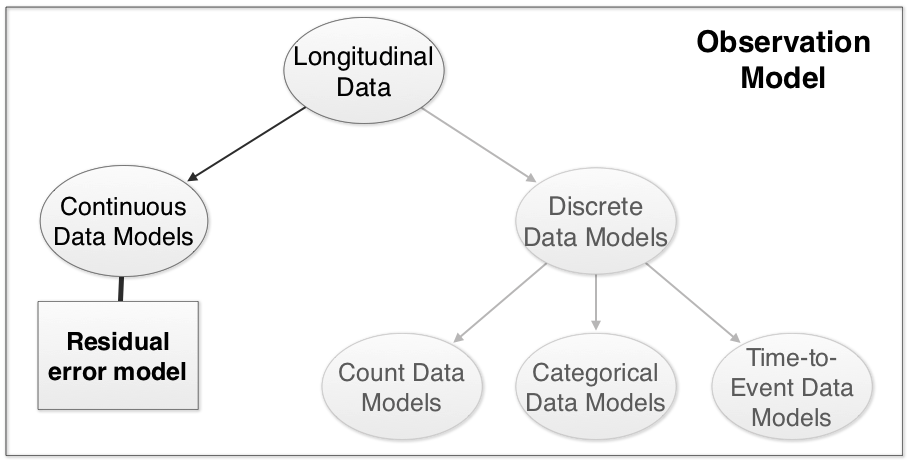
\includegraphics[height=75mm]{observationalModel}
\caption{Observation Model}
\label{fig:observModel}
\end{figure}
An essential component of the Observation Model is the Residual Error Model, which applies only to continuous data models.

%%%%%%%%%%%%%%%%%%%%%%%%%%%%%%%%%%%%%%%%%%%%%%%%%%%%%%%%%%%%%%%%%%
\subsection{Residual error model}
\label{sec:residualErrorModel}
\label{maths:error_model}
\label{maths:combined-err-model}
In this section we consider different forms of the residual error, i.e. this section is about $g$ in the term
\begin{align*}
g(x_{ij}, \psi_{i}, \xi) \epsilon_{ij}
\end{align*}
of eq.\ref{eq:nlmeModel} with $\epsilon_{ij} \sim N(0, 1)$, i.e. a standard normally distributed random variable. We distinguish between
\begin{itemize}\addtolength{\itemsep}{-.95\baselineskip}
\item
models for \textbf{untransformed} data
\begin{align*}
 \underbrace{ y_{ij}}_{\text{\parbox{2cm}{\centering Experimental \\[-4pt]  data}}} =
 \underbrace{ f(x_{ij}, \psi_{i})}_{\text{\parbox{2.5cm}{\centering Model \\[-4pt]  prediction}}} +
 \underbrace{ g(x_{ij}, \psi_{i}, \xi_i) \; \epsilon_{ij}}_{\text{\parbox{3cm}{\centering Residual \\[-4pt] error}}}
 \end{align*}
 \item
\textbf{transform-both-sides} models
\begin{eqnarray}
 \underbrace{ u(y_{ij})}_{\text{\parbox{2cm}{\centering Transformed \\[-4pt] experimental \\[-4pt]  data}}} =
 \underbrace{ u\big(f(x_{ij}, \psi_{i})\big)}_{\text{\parbox{2.5cm}{\centering Transformed \\[-4pt]  model \\[-4pt]  prediction}}} +
 \underbrace{ g(x_{ij}, \psi_{i}, \xi_i) \; \epsilon_{ij}}_{\text{\parbox{3cm}{\centering Residual \\[-4pt] error}}} \nonumber
 \end{eqnarray}
 \item
and \textbf{implicit} models
\begin{eqnarray}
 \underbrace{ u(y_{ij})}_{\text{\parbox{2.5cm}{\centering Transformed \\[-4pt] experimental  data}}} =
 \underbrace{ U\big(f(x_{ij}, \psi_{i}),\xi_i, \epsilon_{1,ij}, \epsilon_{2,ij}, \dots\big)}_{\text{\parbox{2.5cm}{\centering Transformed \\[-4pt]  model prediction}}}
 \end{eqnarray}
\end{itemize}
The \textit{untransformed} form is a special case of the \textit{transform-both-sides} form with $u \equiv Id$, i.e. the identity transformation.
Then for models of both types with $\epsilon_{ij}$ being normally distributed with mean 0 and variance 1, $u(y_{ij})$ is also normally distributed
with mean $u(f(x_{ij}, \psi_{i}))$ and the standard deviation $g(x_{ij}, \psi_{i}, \xi_i)$. \\
Possible extensions to the basic models are
\begin{itemize}
\item
when more than one random variable is applied, i.e. multiple $\epsilon$'s,
\item
when more than one type of measurement or observation is defined, or
\item
when variability, as discussed in section \ref{sec:variabilityModel}, is applied to parameters of the residual error model (see section \ref{subsec:varModelResidualError} for details).
\end{itemize}


%%%%%%%%%%%%%%%%%%%%%%%%%%%%%%%%%%%%%%%%%%%%%%%%%%%%%%%%%%%%%%%%%%
\subsection{Incorporating variability on the residual error model parameters}
\label{subsec:varModelResidualError}
In analogy to the nested hierarchical structure for the variability on the individual parameters,
variability on residual error model parameters can be defined using the same structure.
By doing so, no new structure is necessary to account for any inter-individual and/or inter-occasion variability of the residual error model parameters.

This allows \pharmml to cover the so-called 'ETA-on-EPS' approach -- e.g. IIV on the residual error model parameters or in other words varying residual
error magnitude between individuals, see Figure \ref{fig:IOV0_residualError}.
\begin{figure}[htb!]
\centering
  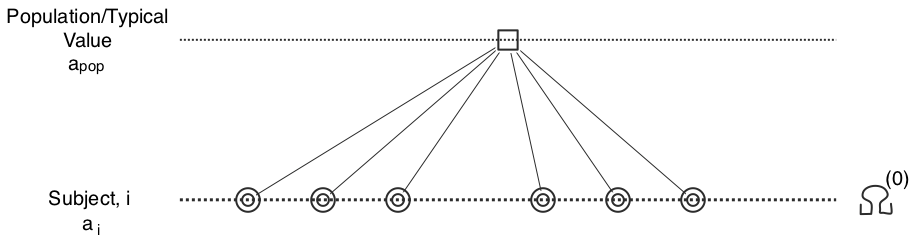
\includegraphics[width=125mm]{pics/IOV0_residualError}
 \caption{Inter-individual variability of the residual error parameter $a$. The nested hierarchical structure is identical to that of structural model parameters.}
 \label{fig:IOV0_residualError}
\end{figure}
For example, if an additive residual error model and a log-normal distribution for $a$ is assumed, then the parameter model reads
\begin{align*}
	& \log(a_i) = \log(a_{pop}) + \eta_a, \quad  \eta_a \sim \mathcal{N}(0,\omega_a^2)
\end{align*}
and the observation model reads
\begin{align*}
	& y_{ij} \sim \mathcal{N}(f_{ij},a_i^2): \quad y_{ij} = f_{ij} + a_i \epsilon_{ij}, \quad \epsilon_{ij} \sim \mathcal{N}(0,1).
\end{align*}
%See also section \ref{modelKK_RM1} for three IIV and IOV examples with NMTRAN and MLXTRAN code.


%%%%%%%%%%%%%%%%%%%%%%%%%%%%%%%%%%%%%%%%%%%%%%%%%%%%%%%%%%%%%%%%%%
\subsection{Residual error model examples}
\label{subsec:modelExamples}
Currently, there is no library of residual error models but this might change in the future. All of the following residual error model examples and their different versions can be implemented in the present version of PharmML:
\begin{itemize}
\item
Constant/additive:
\begin{align*}
& y_{ij} = f_{ij} + a \; \epsilon_{ij}; \quad \epsilon_{ij} \sim N(0,1)  \\
\text{or} \quad & y_{ij} = f_{ij} + \epsilon_{ij}; \quad \epsilon_{ij} \sim N(0,\sigma^2)
\end{align*}
\item
Proportional or constant CV (CCV):
\begin{align*}
&y_{ij} =  f_{ij} + bf_{ij} \; \epsilon_{ij}; \quad \epsilon_{ij} \sim N(0,1)  \\
\text{or} \quad & y_{ij} =  f_{ij}(1+\epsilon_{ij}); \quad \epsilon_{ij} \sim N(0,\sigma^2)
\end{align*}
\item
Combined additive and proportional 1:
\begin{align*}
& y_{ij} =  f_{ij} + (a + bf_{ij}) \; \epsilon_{ij}; \quad \epsilon_{ij} \sim N(0,1)
\end{align*}
\item
Combined additive and proportional 2:
\begin{align*}
& y_{ij} =  f_{ij} + \sqrt{a^2 + b^2f_{ij}^2} \; \epsilon_{ij}; \quad \epsilon_{ij} \sim N(0,1)  \\
\text{or}  \quad & y_{ij} =  f_{ij} +  a\, \epsilon_{1,ij} + b f_{ij}\, \epsilon_{2,ij}; \quad \epsilon_{1,ij} \sim N(0,1); \quad \epsilon_{2,ij} \sim N(0,1);   \\
\text{or}  \quad & y_{ij} =  f_{ij} (1 + \epsilon_{1,ij}) + \epsilon_{2,ij}; \quad \epsilon_{1,ij} \sim N(0,\sigma_1^2); \quad \epsilon_{2,ij} \sim N(0,\sigma_2^2);
\end{align*}
\item
Power error model:
\begin{align*}
& y_{ij} = f_{ij} + b\,f_{ij}^c \; \epsilon_{ij}; \quad \epsilon_{ij} \sim N(0,1)
\end{align*}
\item
Combined additive and power error model 1:
\begin{align*}
& y_{ij} =  f_{ij} + (a + b f_{ij}^c) \; \epsilon_{ij}; \quad \epsilon_{ij} \sim N(0,1)
\end{align*}
\item
Combined additive and power error model 2:
\begin{align*}
& y_{ij} = f_{ij} + a\epsilon_{1,ij} + b f_{ij}^c \epsilon_{2,ij}; \quad \epsilon_{1,ij} \sim N(0,1); \quad \epsilon_{2,ij} \sim N(0,1)
\end{align*}
\item
Two (or more) types of measurements error model:
\begin{align*}
& y_{ij} = f_{ij} + \text{ASY}_j\epsilon_{1,ij} + (1-\text{ASY}_j) \epsilon_{2,ij}; \quad \epsilon_{1,ij} \sim N(0,\sigma_1^2); \quad \epsilon_{2,ij} \sim N(0,\sigma_2^2)
\end{align*}
\item
Two (or more) types of observations error model:
\begin{align*}
& y_{ij} = \text{TYP}_{ij} f_{1,ij} + (1-\text{TYP}_{ij}) f_{2,ij} + \text{TYP}_{ij}\epsilon_{1,ij} + (1-\text{TYP}_{ij}) \epsilon_{2,ij};  \\
&  \epsilon_{1,ij} \sim N(0,\sigma_1^2); \quad \epsilon_{2,ij} \sim N(0,\sigma_2^2)
\end{align*}
%\item
%Extended error model:
%
%y_{ij} = \left\{ \begin{array}{rcl}  f_{ij} + \epsilon_{1,ij}  & \mbox{for} & \text{TIME == 1 \&\& ID == 1} \\
%f_{ij} + \epsilon_{2,ij}  & \mbox{for} & \text{TIME == 2 \&\& ID == 1} \\
%\cdots \end{array}\right\} \quad \text{with} \quad
%\epsilon_{1,ij} \sim N(0,\sigma_1^2),\, \epsilon_{2,ij} \sim N(0,\sigma_2^2), \cdots
%
\end{itemize}
Main sources: \cite{NONMEM:2006aa} and \cite{POPIX:2013}.

\subparagraph{Note 1}
In the list above models are pulled together which have the same variance function.
\subparagraph{Note 2}
Models listed above are the most popular ones in use but the present PharmML structure allows for implementation of virtually any user-defined model. See section ref:XYZ for more examples and PharmML implementation.

%
%%%%%%%%%%%%%%%%%%%%%%%%%%%%%%%%%%%%%%%%%%%%%%%%%%%%%%%%%%%%%%%%%%%
%\subsection{PharmML implementation}
%Some of the above listed residual error model types have two or three equivalent forms, by which we mean they have the same variance, although they use one or more residual errors, $\epsilon_{ij}$. Other types contain two or more predictions from the structural model, \var{f_{ij}}. From a
%computational point of view it makes a lot of sense to reflect such differences in the language structure.
%This was the motivation to allow for the implementation of two types of observation models
%\begin{itemize}
%\item
%\xelem{Standard} -- any observation model of the form
%\begin{align*}
%	u(y_{ij}) = u(f_{ij}) + g\times\epsilon_{ij}
%\end{align*}
%which can be defined using exactly one of the following items
%\begin{itemize}
%\item
%a transformation, $u$, e.g. \var{log} or \var{logit}
%\item
%one structural model prediction, \var{f_{ij}}
%\item
%one standard deviation function, \var{g}
%\item
%one random variable, $\epsilon_{ij}$
%\end{itemize}
%\item
%\xelem{General} -- using any number of the items listed above and arbitrary functional relationship between them.
%\end{itemize}
%Chapter \ref{chap:worked-egs} contains a number of examples illustrating these constructs.

%\begin{itemize}
%\item
%standard -- defined in the spec as \xelem{Standard} with following child elements
%\begin{itemize}
%\item
%\item
%\item
%\end{itemize}
%\item
%general -- defined in the spec as \xelem{General}.
%\end{itemize}




%The residual errors are part of the \textit{Observations Model}, see section \ref{sec:eg1-obs-model} for detailed discussion.
%The following table contains some of the models which can be implemented in \pharmml:
%
%\begin{table}[htdp]
%\begin{center}
%\begin{tabular}{l c c}
%Model name & $g$ & $\xi$ \\
%\hline \hline
%Constant error model & $a$ & $a$ \\
%Proportional error model & $bf$ & $b$ \\
%Combined error model & $a + bf$ & $a,b$ \\
%Alternative combined error model 1& $\sqrt{a^2 + b^2f^2}$ & $a,b$ \\
%Alternative combined error model 2 & $a + bf^c$ & $a, b, c$
%\end{tabular}
%\end{center}
%\caption{Examples of residual error models which can be implemented in \pharmml.}
%\label{tab:residualModels}
%\end{table}%




